\documentclass[12pt]{IEEEtran}
\IEEEoverridecommandlockouts
\usepackage{fancyhdr}
\usepackage{graphicx}
\usepackage[spanish, es-tabla, es-nodecimaldot]{babel}
% \usepackage[utf8]{inputenc}
\usepackage{color}
\usepackage{csquotes}
\usepackage{wrapfig}
\usepackage[l3]{csvsimple}
\usepackage{array}
\usepackage[calc, spanish]{datetime2}
\usepackage{enumitem}
% \usepackage{multicol}
\usepackage{chemformula}
\usepackage{multirow}
\usepackage{mismath}
\usepackage{adjustbox}
\usepackage{nccmath}
\usepackage{amsmath}
\usepackage{amssymb}
\usepackage{mathtools}
\usepackage{amsfonts,latexsym} % para tener disponibilidad de diversos simbolos
\usepackage{enumerate}
\usepackage{empheq}
\usepackage{booktabs}
\usepackage{derivative}
\usepackage{float}
\usepackage{threeparttable}
\usepackage{array,colortbl}
\usepackage{ifpdf}
\usepackage{rotating}
\usepackage{stfloats}
\usepackage{tabularray}
\usepackage{url}
\usepackage{listings}
% \usepackage[inline]{showlabels}
\usepackage{kantlipsum}
\usepackage{siunitx}
\usepackage{amsmath}
\usepackage{makecell}%To keep spacing of text in tables
\setcellgapes{2pt}%parameter for the spacing in tables
\usepackage{afterpage}
\usepackage[
  sorting=none,
  backend=biber,
  style=ieee,
  % bibstyle = authoryear,
  citestyle=numeric-comp,
]{biblatex}
\usepackage{hyperref}
\usepackage{cleveref}
\crefname{table}{tabla}{tablas} % Table's cross-reference name
\crefname{equation}{ec.}{ecs.} %
\newcommand\crefrangeconjunction{--}
\newcommand\crefpairconjunction{~y~}
\providecommand{\abs}[1]{\lvert#1\rvert}
%%%%%%%%%%%%%%%%%%%%%%%%%%%%%%%%%%%%%%%%%%%
%%% CREAR Y REESCRIBIR ALGUNOS COMANDOS %%%
%%%%%%%%%%%%%%%%%%%%%%%%%%%%%%%%%%%%%%%%%%%
\newcolumntype{P}[1]{>{\centering\arraybackslash}p{#1}}  %% Se crea un nuevo tipo de columna llamada P.
\newcommand{\tabitem}{~~\llap{\textbullet}~~}
\newcommand{\ctt}{\centering\scriptsize\textbf} %%\ctt abrevia el comando \centering\scriptsize\textbf
\newcommand{\dtt}{\scriptsize\textbf} %%\dtt abrevia el comando \scriptsize\textbf
\renewcommand\IEEEkeywordsname{Palabras clave}

%% Crea una lista en dos columnas
\SetEnumitemKey{twocol}{%
  itemsep = 1\itemsep,
  parsep = 0.5\parsep,
  before = \raggedcolumns
  \begin{multicols}{2},
    after =
\end{multicols}}
%%%%%%%%%%%%%%%%%%%%%%%%%%%%%%%%%%%%%%%%%%%

% correct bad hyphenation here
\hyphenation{op-tical net-works semi-conduc-tor} %% Con este comando se especifican como pueden seprarse las sílabas adecuadamente en caso una palabra quede en dos lineas diferentes de texto

\graphicspath{ {figs/} {logos/}}  %%Ruta donde se encuentran las imágenes, que esté vacio indica que las imagenes están dentro de la misma carpeta que contiene el archivo .tex

\sisetup{
  output-decimal-marker = {.},
  uncertainty-mode = separate,
}
% adjust as needed
\addtolength{\footskip}{0\baselineskip}
\addtolength{\textheight}{-1\baselineskip}

%Paquete tikz para hacer diagramas y figuras
\usepackage{tikz}
\usetikzlibrary{arrows}
%\usepackage[spanish,es-noquoting]{babel}

%%%%%%%%%%%%%%%%%%%%%%%%%%%%%%%%
%%%%% INICIO DEL DOCUMENTO %%%%%
%%%%%%%%%%%%%%%%%%%%%%%%%%%%%%%%

\addbibresource{bibliography.bib}

\DTMsavedate{duedate}{2024-02-25}% Año-Mes-Día -> Fecha de entrega
\DTMnewdatestyle{usvardate}{%
  \renewcommand{\DTMdisplaydate}[4]{%
    \DTMMonthname{##2}\nobreakspace% Mes
    \number##1% Año
  }%
  \renewcommand{\DTMDisplaydate}{\DTMdisplaydate}%
}

\begin{document}
%%%%%%%%%%%%%%%%%%%%%%%%%%%%
%%% TÍTULO DEL DOCUMENTO %%%
%%%%%%%%%%%%%%%%%%%%%%%%%%%%

\title{Efecto fotoeléctrico}

%%%%%%%%%%%%%%%%%%%%%%%%%%%
%%%%%%%%% AUTORES %%%%%%%%%
%%%%%%%%%%%%%%%%%%%%%%%%%%%

\author{\IEEEauthorblockN{Jesus Diego Gomez Garnica, Marcos López Merino}\\
  \IEEEauthorblockA{\textbf{Profesor}: Alejandro Rosado Fuentes}\\
\IEEEauthorblockN{\DTMusedate{duedate}}}

%%%%%%%%%%%%%%%%%%%%%%%%%%%
\twocolumn[
  \begin{@twocolumnfalse}
    \maketitle
    \begin{abstract}
        Mediante el estudio del efecto fotoeléctrico se buscó estimar la constante de Planck \(h\) y la función de trabajo \(\phi\) del antimoniuro de cesio (\ch{Cs3Sb}). Para ello, se caracterizó el espectro de emisión del mercurio identificando sus picos principales y se incidió la radiación correspondiente a cada una de estas longitudes de onda hacia un fototubo IP39, con la intención de determinar el potencial de frenado \(V_{0}\). Finalmente, a partir de la relación lineal entre el potencial de frenado \(V_{0}\) y la frecuencia de la radiación incidente \(\nu\), dada por \(V_{0} = \tfrac{h}{\mathrm{e}}\nu - \tfrac{\phi}{\mathrm{e}}\), se intentó determinar los valores de \(h\) y \(\phi\). Sin embargo, los datos experimentales obtenidos para el potencial de frenado no permitieron obtener resultados precisos, lo que sugiere la presencia de errores significativos en la medición de las corrientes.
    \end{abstract}
  \end{@twocolumnfalse}
  \vspace{1cm}
]

%%%%%%%%%%%%%%%%%%%%%%
%\IEEEpeerreviewmaketitle
%%%%%%%%%%%%%%%%%%%%%%%%%%%%%%%%%%%%%
%%% PRIMERA SECCIÓN DEL DOCUMENTO %%%
%%%%%%%%%%%%%%%%%%%%%%%%%%%%%%%%%%%%%
\section{Introducción}

El efecto fotoeléctrico ocurre cuando una superficie metálica es iluminada y se desprenden electrones, llamados fotoelectrones. Este fenómeno fue observado por primera vez por Heinrich Hertz en 1887 mientras realizaba experimentos sobre la radiación electromagnética.\cite{kraneModernPhysics2019a} 
La \cref{fig:photoelectric-circuit} muestra el arreglo experimental usado para estudiar el efecto fotoeléctrico. Un fototubo con dos electrodos conectados a una fuente de voltaje, donde la superficie en la que incide la luz es el fotocátodo. Algunos de los fotoelectrones que se desprenden de la superficie metálica tiene suficiente energía para alcanzar el ánodo, generando una corriente eléctrica. \cite{tiplerModernPhysics2012} La máxima energía de los fotoelectrones puede medirse aplicando una diferencial de potencial \(\Delta V\) entre el fotocátodo y el ánodo que determina si los fotoelectrones alcanzan el ánodo o no. A medida que \(\Delta V\) aumenta, incluso los electrones más energéticos no poseen la energía cinética suficiente para alcanzar el ánodo. El potencial con el que se reduce la corriente a cero se conoce como \emph{potencial retardador} o \emph{de frenado} \(V_{0}\) y está relacionado con la energía cinética máxima de los fotoelectrones mediante la siguiente expresión\cite{kraneModernPhysics2019a, beiserConceptsModernPhysics2003},

\begin{equation}
    K_{\text{máx}} = \mathrm{e}V_{0}.
    \label{eq:k-max}
\end{equation}

\begin{figure}[htp]
    \centering
    \includegraphics[width=\linewidth]{photoelectric-circuit.pdf}
    \caption{Circuito del arreglo experimental.\cite{EfectoFotoelectrico}}
    \label{fig:photoelectric-circuit}
\end{figure}

En 1905, Einstein propuso una explicación sobre la independencia del potencial de frenado de la intensidad de la luz, asumiendo que la cuantización usada por Planck era una característica universal de la luz. Es decir, la luz consiste de cuantos de luz, denominados fotones, cada uno con energía

\begin{equation}
    E = h\nu,
    \label{eq:photon-energy}
\end{equation}

donde \(h\) es una constante de proporcionalidad conocida como la constante de Planck, cuyo valor aceptado es de \qty{6.6260696e-34}{\J\s}.

Cuando un fotón incide sobre la superficie del fotocátodo, toda su energía es absorbida por un solo electrón. Si la energía necesaria para remover un electrón de la superficie metálica es \(\phi\), entonces la energía máxima de ese fotoelectrón es \(h\nu - \phi\), esto como consecuencia de la conservación de la energía. Entonces, la ecuación del efecto fotoeléctrico es

\begin{equation}
    V_{0} = \dfrac{h}{\mathrm{e}}\nu - \dfrac{\phi}{\mathrm{e}},
    \label{eq:photoelectric}
\end{equation}

donde la función de trabajo para el antimoniuro de cesio está en el rango de \(\phi = \qtyrange[range-phrase=\text{--}]{1.6}{1.8}{\eV}\)\cite{sakataStudiesCs3SbPhotoCathode1953,caulfieldCesiumAntimonyFilms1966}.

\section{Aplicación a la industria}
%\kant[2]

El efecto fotoeléctrico es fundamental en la innovación de nuevas tecnologías, este posee aplicaciones en industrias clave. Por profundizar en una de ellas, los paneles solares \cite{panelessolaresfotovoltanicos} se convirtieron en una fuente alternativa de obtención de energía eléctrica, al estar compuestos por células fotovoltaicas, generalmente hechas de silicio, estas absorben fotones de la luz solar liberando un flujo de electrones que se canaliza a través de un circuito, produciendo energía utilizable. Gracias a este proceso, los paneles solares son una fuente limpia de electricidad, ampliamente utilizada en hogares, industrias y proyectos de energía a gran escala.

Sin embargo, no es la única utilidad, el efecto fotoeléctrico se puede encontrar en los sensores de luz en cámaras, sistemas de seguridad, lectores de código de barras o cosas mucho mas especializadas, como foto multiplicadores para detectar radiación, instrumentos para estudiar espectros estelares o en medicina para las radiografías digitales, todas estas formas prácticas de utilizar este conocimiento, han hecho que su versatilidad ademas de su eficiencia lo conviertan en un pilar de la innovación industrial y científica.

\section{Procedimiento experimental}

Para la realización de la práctica se requiere de una fuente de luz de mercurio \emph{PASCO OS-9286A} \cite{InstructionSheetPASCO}, un monocromador \emph{SPEX MINIMATE}, un fototubo IP39, un multímetro \emph{Steren MUL-050} \cite{STERENMUL050MANUAL}, una fuente de voltaje y un electrómetro \emph{Keithley 610B} \cite{Keithley610B} en un arreglo como se muestra en la \cref{fig:photoelectric-arrangement}.

\begin{figure}[htp]
    \centering
    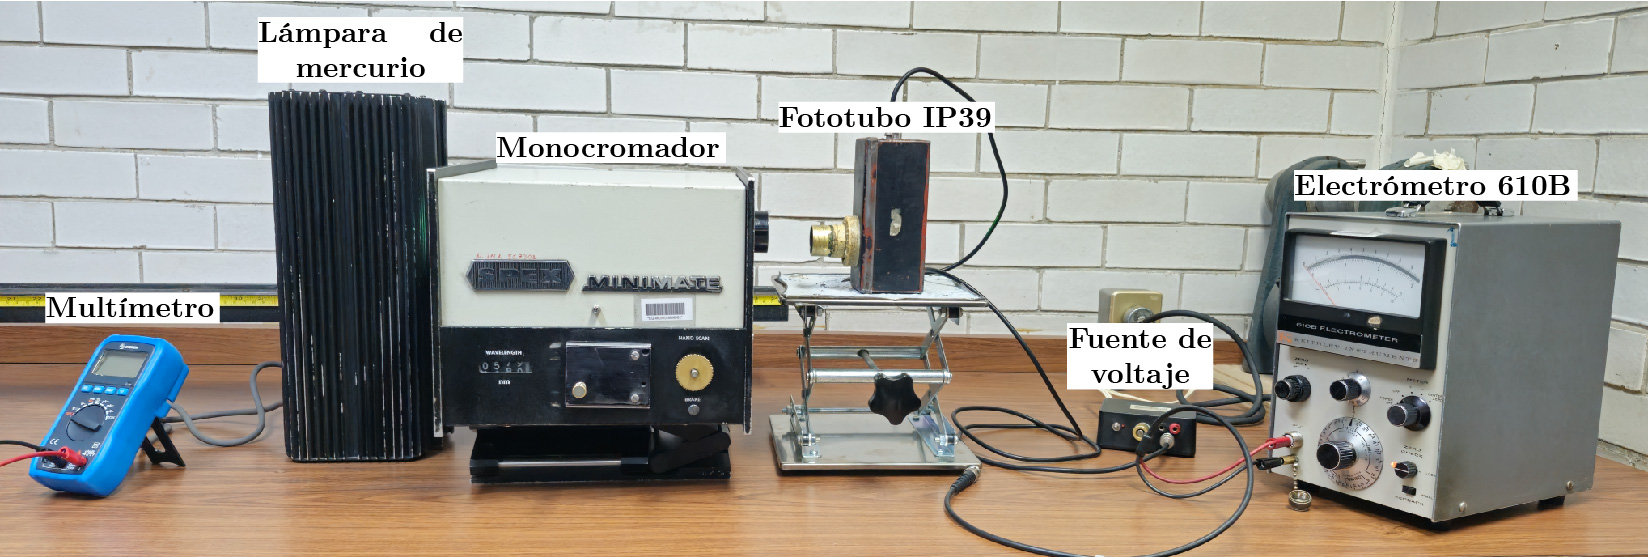
\includegraphics[width=\linewidth]{montaje-experimental}
    \caption{Montaje experimental para observar el efecto fotoeléctrico.}
    \label{fig:photoelectric-arrangement}
\end{figure}

Como pasos preliminares se conectan por \qty{30}{\minute} y \qty{10}{\minute} el electrómetro y la fuente de mercurio, respectivamente. El primero para disminuir el desplazamiento de la aguja y el segundo para obtener el espectro de emisión del mercurio con la mayor intensidad.


\subsection{Espectro de emisión del mercurio}

Se realizó un barrido de las longitudes de onda, de \qtyrange[range-phrase = --]{300}{800}{\nm} con incrementos de \qty{10}{\nm}, manteniendo un voltaje constante de \qty[separate-uncertainty-units = bracket]{4.00(3)}{\V}. Para cada longitud de onda, se registró el valor de la corriente correspondiente. A partir de este espectro, se identifican las longitudes de onda con mayor intensidad, las cuales se utilizarán para determinar el potencial de frenado.

\subsection{Voltaje de frenado}

Para cada una de las longitudes de onda identificadas, \qtylist[separate-uncertainty-units = bracket]{340(5);440(5);550(5);580(5)}{\nm}, se varió el voltaje en el rango de \qtyrange{-5}{5}{\V}, en pasos de \qty{0.5}{\V}, registrando las corrientes correspondientes. El valor del voltaje de frenado \(V_{0}\) es el voltaje para el cual la corriente medida es cero.

Las datos de longitudes de onda y voltajes de frenado \(V_{0}\) obtenidos serán utilizados para determinar la constante de Planck y la función de trabajo del metal.

\section{Resultados y análisis}

\subsection{Espectro de emisión del mercurio}

Una vez identificadas las longitudes de onda de las líneas espectrales más intensas obtenidas experimentalmente (\cref{fig:espectro-exp}) se compararon con las mostradas en el espectro de emisión que se incluye en el manual de la lámpara de mercurio, así como las registradas en \cite{MercurySpectra}, para determinar y elegir las longitudes de ondas adecuadas (\cref{fig:espectro-manual}). \\

\begin{figure}[htp]
    \centering
    \includegraphics[width=\linewidth]{espectro-mercurio}
    \caption{Espectro de emisión del mercurio obtenido experimentalmente con las incertidumbres correspondientes al monocromador y al electrómetro.}
    \label{fig:espectro-exp}
\end{figure}

\begin{figure}[htp]
    \centering
    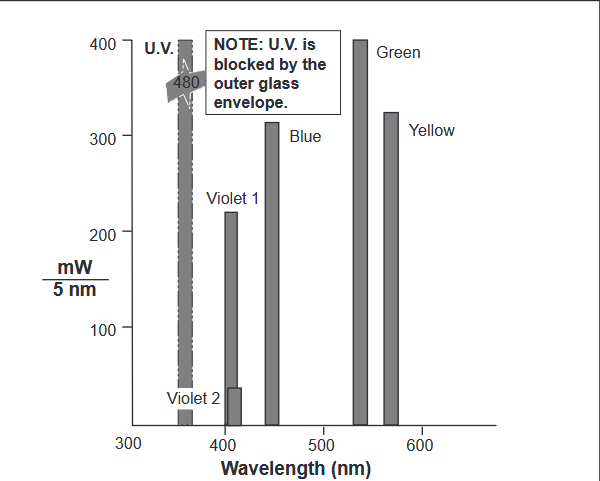
\includegraphics[width=\linewidth, trim={0 0 0.5cm 0.5cm},clip]{espectro-manual}
    \caption{Espectro de emisión del mercurio mostrado en \cite{InstructionSheetPASCO}.}
    \label{fig:espectro-manual}
\end{figure}

Posteriormente, se calcularon las frecuencias asociadas a partir de la relación entre la longitud de onda y la frecuencia, \emph{i.e.},

\begin{equation}
    \nu = \dfrac{c}{\lambda},
\end{equation}

con \(c\) la velocidad de la luz. Esto sera de gran ayuda para ajustar la gráfica a la recta esperada


\subsection{Voltaje de frenado}

Para cada longitud de onda seleccionada, se midió la corriente en función del voltaje aplicado al fototubo dando por resultado la \cref{fig:corriente-voltaje}.

\begin{figure}[htp]
    \centering
    \includegraphics[width=\linewidth, trim={0 0 0.5cm 0.5cm},clip]{figs/corriente-voltaje.png}
    \caption{Corrientes obtenidas a partir la las longitudes de onda deseadas.}
    \label{fig:corriente-voltaje}
\end{figure}

El comportamiento lineal de la corriente con el voltaje sugiere que la luz no incidía únicamente en el fotocátodo. Esto puede deberse a una incorrecta alineación del monocromador con el fototubo o al ruido en las mediciones de las corrientes del electrómetro. El comportamiento para esta gráfica debería ser similar a una sigmoide; sin embargo, se observa el comportamiento esperado por la ley de Ohm.

\subsection{Constante de Planck y función de trabajo}

Una vez catalogados los potenciales de frenado, estos pasan por un proceso de ajuste por regresión de distancia ortogonal (ODR)\cite{mastrandreaErrorAmbasVariables} pues cada uno de los datos tiene un error asociado: al multímetro para el voltaje de frenado y a la propagación de incertidumbres para la frecuencia. Los resultados se muestran en la \cref{fig:potencial-frecuencia}.

\begin{figure}[htp]
    \centering
    \includegraphics[width=\linewidth, trim={0 0 0.5cm 0.5cm},clip]{figs/potencial-frecencia.png}
    \caption{Gráfica de los datos obtenidos experimentalmente de \(V_{0}\) vs \(\nu\), así como la gráfica que resulta del ajuste por ODR de estos.}
    \label{fig:potencial-frecuencia}
\end{figure}

A partir de este ajuste se puede estimar la constante de Planck y la función de trabajo del metal, como se segmenta de la \cref{eq:photoelectric} sabemos que la pendiente de la recta corresponde a \(h/\mathrm{e}\) y su ordenada al origen a \(\phi/\mathrm{e}\), respectivamente. De esta manera, \(h = \qty[separate-uncertainty-units = bracket]{7.279(8.608)e-35}{\J\s}\) y \(\phi = \qty[separate-uncertainty-units = bracket]{1.178(5.539)e-20}{\eV}\), los cuales fueron comparados con sus respectivos valores teóricos a través de la siguiente expresión,

\begin{equation}
    \delta = \abs{\dfrac{v_{A}-v_{E}}{v_{E}}}\cdot 100\%,
\end{equation}

donde $v_{A}$ es valor experimental observado, $v_{E}$ es el valor teórico y $\delta$ el error porcentual. El error porcentual obtenido para la constante de Planck fue de $89\%$ respecto al valor teórico. Esta diferencia sugiere la presencia de errores, como una incorrecta selección de las longitudes de onda o imprecisiones en la medición de las corrientes. Por otro lado, el valor experimental obtenido para la función de trabajo \(\phi\) no se encuentra dentro del rango esperado \qtyrange[range-phrase=\text{--}]{1.6}{1.8}{\eV} según la literatura \cite{sakataStudiesCs3SbPhotoCathode1953,caulfieldCesiumAntimonyFilms1966}, lo que refuerza los posibles errores mencionados más arriba.

\section{Conclusiones}
%\kant[5]
El efecto fotoeléctrico es una demostración clásica de la física cuántica que permite estimar la constante de Planck y la función de trabajo asociado a los conductores eléctricos.

Este experimento representa un reto en su instrumentación. La importancia de tener una certera precisión de las frecuencias y su una correcta alineación de la luz incidente sobre el fototubo IP39 es indispensable para obtener el voltaje de frenado, fundamental para medir la constante de Planck. Así como un mayor conocimiento sobre el funcionamiento preciso del electrómetro para cerciorarse que las medidas de corriente sean las adecuadas.

Las mediciones tomadas de parte del experimento representan un error considerable respecto al valor de la constante de Planck el cual se buscaba precisar, esto puede deberse a la inexactitud en la que la longitud de onda  aislada de la fuente de luz de mercurio no incidiera unicamente en el cátodo del fototubo, lo que provocó no poder medir con precisión el potencial de frenado para cada frecuencia y por ende aumentar error porcentual respecto al valor teórico buscado.


%%%%%%%%%%%%%%%%%%%%%%%%%%%%%%%%
%%%%%%    Bibliografia   %%%%%%%
%%%%%%%%%%%%%%%%%%%%%%%%%%%%%%%%
% \newpage
\nocite{*}
\printbibliography
%\section{Apéndices}
%\appendices

\end{document}
%%%%%%%%%%%%%%%%%%%%%%%%%%%%%%%%
%%%%%% FIN DEL DOCUMENTO %%%%%%%
%%%%%%%%%%%%%%%%%%%%%%%%%%%%%%%%
